\documentclass[]{aastex62}
\usepackage{amssymb,amsmath}

 
\newcommand{\vk}{von K\'{a}rm\'{a}n}
\newcommand{\vdag}{(v)^\dagger}
\newcommand\aastex{AAS\TeX}
\newcommand\latex{La\TeX}


\def\eq#1{\begin{equation} #1 \end{equation}}
\def\mic              {\hbox{$\mu\mathrm{m}$}}
\def\atm    {\hbox{\rm{ATM}}}
\def\dC     {\hbox{$^{o}C$}}
\graphicspath{{./}{figures/}}

%% Reintroduced the \received and \accepted commands from AASTeX v5.2
%\received{May 7, 2019}
%\revised{May 8, 2019}
%\accepted{--}
%% Command to document which AAS Journal the manuscript was submitted to.
%% Adds "Submitted to " the arguement.
%\submitjournal{Icarus}

\shorttitle{Variation of CubeSat Temperature along its Orbit}
\shortauthors{}

\begin{document}

\title{A Simple Model for the Variation of CubeSat Temperature along its Orbit}  
 
%\email{ivezic@uw.edu}

\author[0000-0001-5250-2633]{\v{Z}eljko Ivezi\'{c}}
\affiliation{Department of Astronomy, University of Washington, 3910 15th Avenue NE, Seattle, 
                      WA 98195, USA; e-mail: ivezic@uw.edu}

\begin{abstract}
We discuss a simple model for the variation of CubeSat temperature along its orbit. First 
we consider an analytic solution for the satellite temperature variation with time when subjected to 
a bistable heat source: two segments with piece-wise constant power, such as orbits with an eclipsed 
segment when the Sun is not directly visible. The model assumes that at a given time a single 
temperature applies to the entire satellite body. Discussion is focused on CubeSat satellites in 
low-Earth orbits, the uncertainties in predicted temperatures due to uncertain input parameters, and 
it emphasizes the importance of the satellite thermal inertia in setting the amplitude of the temperature 
variation along the orbit. This simplified ``spherical cow'' model is suitable for studying the relative 
effects of surfaces with different emissivities, the effects of small changes in the solar flux between 
June and December, the impact of thermal inertia, and as a ``sanity check'' for the results obtained 
with numerical thermal models that utilize detailed geometrical and thermal descriptions of all satellite 
components. We also developed a numerical model with arbitrary time dependence of the heating power, including its 
dependence on the satellite temperature, and validated it using analytic solution for a bistable heat 
source. Analysis of a typical 2U CubeSat shows that low temperatures are more worrisome than
high temperatures, and that low temperatures can be mitigated by active temperature control such
as releasing heat when the satellite is in eclipse using electrical energy stored in batteries that
are charged during non-eclipsed portion of the orbit. 
\end{abstract}

\keywords{Satellites --- CubeSat --- Radiative transfer -- Analytic solution}


\section{Introduction} 
 
Over the last two decades, the concept of a small modular satellite named CubeSat\footnote{For more 
details and references, see https://en.wikipedia.org/wiki/CubeSat} has become
extremely popular -- to date about two thousand satellites were launched or are in preparation 
stage\footnote{See https://en.wikipedia.org/wiki/List\_of\_CubeSats}. CubeSat projects have both
scientific and educational values, and are suported by many universities as well as space organizations
such as NASA and ESO. 

When designing a satellite, it is crucial to establish that the temperature variation for each component 
will be within its operating range. In practice, professional engineering tools (such as Ansys framework)
and numerical analysis are used to analyze complex systems. Nevertheless, approximately correct temperature estimates 
and physical insight can be derived even using simple analytic models. Such models can be used as
a ``sanity check'' for the results obtained with complex thermal models that include 
numerous input parameters, and for fast input parameter exploration (e.g., runtime for a numerical 
transient model using the Ansys code can be several hours). Simplified models are also useful as an
educational tool and they help develop deeper physical understanding than numerical simulations. 

While there is relatively abundant literature on CubeSat thermal modeling, it appears that a 
compact reference appropriate for undergraduate and graduate students entering this field,
and supported by easy to use open source code, has not been published yet. This paper is
attempting to fill this gap and it is a result of our work with two CubeSat projects:  the SOC-i satellite project\footnote{https://www.aa.washington.edu/news/article/2019-02-11/cubesat-team}
at the University of Washington and the Perun satellite project\footnote{https://perun-i.hr/en/} in Croatia.  

A simple model for the satellite temperature variation with time can be derived by assuming that a single
temperature applies to the entire satellite body at any  given time. An implication of this assumption is 
that the thermal resistivity across the surface is vanishing and thus the entire surface can reach the
same temperature very quickly (under a minute or less). This model permits an analytic solution 
when subjected to a bistable heat source with two segments that each have constant input power 
(the sum of input heating flux and internal power dissipation). A bistable heat source is a good 
approximation for a satellite orbit with an eclipsed segment when the Sun is not directly visible. 

The governing equations for such a simple model with bistable heat source are presented in the 
following Section, and numerical results are discussed in Section 3.  In Section 4 we discuss
active temperature control and summarize our conclusions in Section 5. 


\section{Simple single-temperature thermal model} 

Consider a satellite with a given geometry and assume a uniform temperature over its surface
at any given time, $T(t)$. The temperature variation with time depends on the difference between
heat source, $Q_{in}$, and heat sink, $Q_{out}$, 
\eq{
\label{eq:dTdt}
                 m C {dT \over dt} =  Q_{in} - Q_{out}, 
}
where $m$ is the satellite mass and $C$ is the material heat capacity. The heat capacity for 
most common materials used in satellites is listed in Table~\ref{tab:inputsMatProp}. 
The $mC$ product is often called the thermal inertia. Heat sources and sinks are measured in 
Watts (W = Js$^{-1}$). 

\begin{table}[ht!]
	\centering
	\caption{Common material properties (Gilmore 2002). }
	\label{tab:inputsMatProp}
	\begin{tabular}{r|r|r|r} % 
		\hline
  	        Material    &      density &   specific heat & thermal conductivity \\
		\hline
                 \phantom{x}              & $\rho$ (kg\,m$^{-3}$)   &   $C$ (J\,kg$^{-1}$\,K$^{-1}$)  & $k$ (W\,m$^{-1}$\,K$^{-1}$)  \\
             Aluminum  &       2,710       &         768--921      &     120--205  \\ 
             Solar cells  &       2,285       &         300--700      &     60--100    \\
 		\hline
	\end{tabular} 
      % $^a$ $\rho$ is mass density, $C$ is heat capacity (specific heat), and $k$ is thermal conductivity. 
\end{table}
 
\subsection{Radiative heat sink} 

Assuming that the satellite is in vacuum, the heat sink is due to radiative losses
\eq{
\label{eq:Qout}
                      Q_{out} = A_{tot} \epsilon_T \, \sigma T^4  
}
where $A_{tot}$ is the satellite total surface area (e.g., for a spherical satellite $A_{tot} = 4\pi R^2$,
where $R$ is the satellite radius), $\sigma=5.67\times10^{-8}$ Wm$^{-2}$K$^{-4}$ is the Stefan-Boltzmann 
constant,  and $\epsilon_T$ is the wavelength-averaged surface emissivity over the thermal flux distribution. 
The surface emissivity $\epsilon_T$ is approximately equal to the emissivity at the wavelength of the peak emission. From Wien's 
law, this wavelength is equal to (3000 K$\mic$)/T and thus for $T \approx 300$ K, $\epsilon_T$ is approximately 
equal to the material emissivity around 10 $\mic$. Typical values of $\epsilon_T$  for materials used in 
satellite industry are in the range 0.8-0.9; values of $\epsilon_T$ for common materials are listed in 
Table~\ref{tab:inputsAbsEmiss}. 

The energy spent on battery charging (the conversion of incoming solar flux to chemical energy) is 
also a heat sink. However, essentially all of that energy is returned back as a heat source at a later time. 
The treatment of these effects is discussed separately further below (see \S~\ref{sec:batteries}). 


\begin{table}[t]
	\centering
	\caption{Surface optical absorptivity and infrared emissivity (Gilmore 2002). }
	\label{tab:inputsAbsEmiss}
	\begin{tabular}{r|r|r} % 
		\hline
  	                  Surface       &    $\alpha_S$  &   $\epsilon_T$    \\
		\hline
  Black anodized aluminum  &       0.86      &         0.86     \\ 
    Blue anodized aluminum  &       0.67      &         0.86     \\ 
 Yellow anodized aluminum  &       0.47     &         0.86     \\ 
   Solar panels                      &        0.92     &         0.85     \\
   Black plastic                     &       0.95       &         0.87     \\ 
   Catalac White Paint          &        0.24      &         0.90      \\ 
   Dupont Silver Paint        &          0.43      &         0.49      \\
   Buffed Aluminum           &          0.16      &         0.03      \\  
    Buffed Copper               &          0.30      &         0.03      \\  
  Polished stainless steel   &         0.42        &        0.11     \\ 
      Gold coating                &        0.19        &       0.02       \\
     Kapton foil                    &       0.11         &        0.33      \\
		\hline
	\end{tabular} 
\end{table}



\subsection{Heat sources} 

The heat sources can include direct solar radiation, $Q_{sun}$, solar radiation reflected from Earth, 
$Q_{ref}$, and thermal infrared emission from Earth, $Q_{IR}$. When the satellite is exposed to direct 
sunlight, the maximum possible heat source corresponds to 
\eq{
\label{eq:QinSun} 
                   Q_{in}^{sun}  = Q_{sun} + Q_{ref} + Q_{IR}  
} 
while the minimum possible heating corresponds to 
\eq{
\label{eq:QinEclipse} 
                     Q_{in}^{eclipse}  = Q_{IR},
} 
when the satellite is in Earth's shadow (eclipsed by Earth). For illustration, see figure~\ref{fig:JacquesFig22}. 

%The two extremes, ``hot'' and ``cold'', should not be confused with ``hot'' and ``cold'' scenarios
% that maximize/minimize the satellite temperature over an orbital cycle. 
 

\begin{figure}[t]
\centering
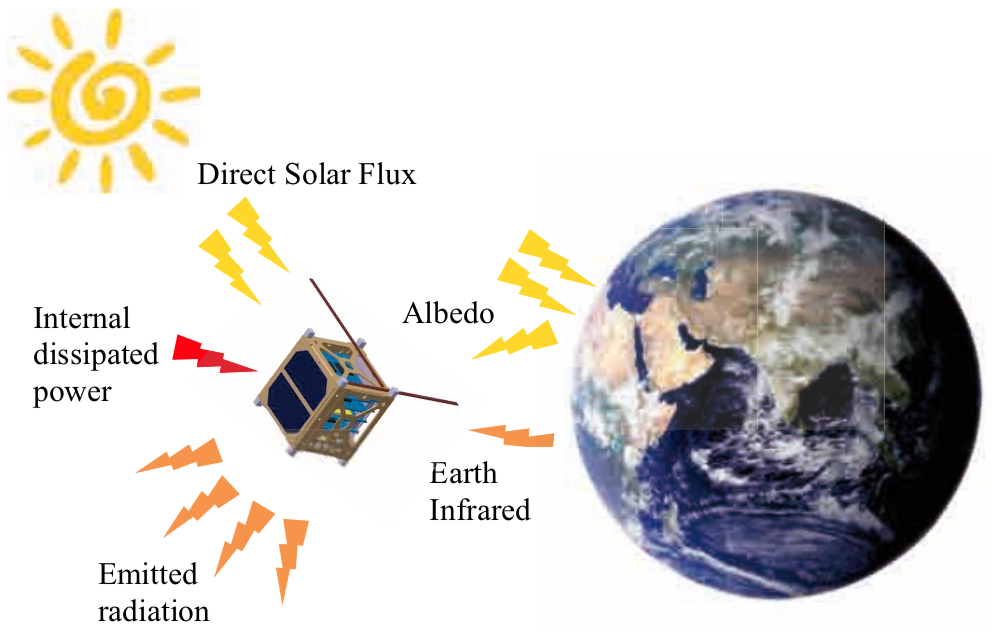
\includegraphics[width=0.65\textwidth, keepaspectratio]{figures/Jacques_heatSources.png} 
\caption{An illustration of the satellite heat balance (here 1U CubeSat satellite is shown). 
The heat sources include direct solar radiation, solar radiation reflected from Earth (albedo), 
infrared radiation emitted by Earth, and internally dissipated power. Conversion of input
radiation to chemical energy in batteries is not shown. The heat sink is thermal infrared radiation 
emitted by the satellite and energy for battery charging. Credit: Figure 2.2 from the master thesis 
by Lionel Jacques (2009, University of Liege). 
\label{fig:JacquesFig22}}
\end{figure}


\subsubsection{Solar radiation} 

The time-averaged solar flux is about $F_{sun}$=1372 Wm$^{-2}$ and its spectral energy distribution peaks 
at wavelenghts of about 0.5 $\mic$ (yellow light; the Sun's surface temperature is about 5,800 K). Since 
Earth's orbit is not circular, the solar flux varies from 1322 Wm$^{-2}$ in June to 1422 Wm$^{-2}$ in December, 
or by about 4\% around its mean value (see Table~\ref{tab:inputsEnvParam}). The absorbed energy due to 
solar flux is then 
\eq{
\label{eq:Qsun}
                   Q_{sun}  = A_S \, \alpha_S  \, F_{sun} = \eta_S \, A_{tot} \, \alpha_S  \, F_{sun} 
} 
where  $A_S$ is the satellite's mean projected surface area towards the Sun (for sphere, $A_S = \pi R^2$ and
$\eta_S=1/4$), and $\alpha_S$ is the wavelength-averaged surface absorptivity over the solar flux distribution. 
Following Kirchhoff's law, absorptivity $\alpha_S$ is approximately equal to the emissivity at 0.5 $\mic$, the wavelength 
of the peak of the solar spectral energy distribution\footnote{The following convention is used in ESA and NASA 
literature: $\epsilon$ is the mean emissivity (and absorptivity) in the infrared wavelength range (5--35 \mic), 
and $\alpha$ is the mean absorptivity (and emissivity) in the optical wavelength range (0.3--2.4 \mic).}. The low 
values of $\alpha_S$ imply high reflectivity and ``shiny'' surfaces. The values of  $\alpha_S$ for common 
materials are listed in Table~\ref{tab:inputsAbsEmiss}. 
 

\begin{table}[t]
	\centering
	\caption{The range of input enviromental parameters. }
	\label{tab:inputsEnvParam}
	\begin{tabular}{r|r|r|r|r} % 
		\hline
  	         Quantity & max    &   min   &  mean &  unit            \\
		\hline
              Solar flux   &  1422  &  1322  &  1372 & Wm$^{-2}$  \\
           Earth albedo  &    35    &    25    &     30  &   \%            \\ 
            Earth IR flux &  260    &   220   &    240 & Wm$^{-2}$   \\
 		\hline
	\end{tabular} 
\end{table}

\subsubsection{Solar radiation reflected from Earth} 

 
The fraction of solar flux reflected by Earth back towards the satellite is typically $\rho_E=0.3$, and it 
varies in the range $\rho_E=0.2-0.4$ across Earths' surface and oceans. The reflected flux depends on the
"Sun-Earth-satellite" angle, $\theta$, and it is maximized when the satellite is at the subsolar point. 
Gilmore (2002) gives an approximate formula for the variation of reflected light with $\theta$ as 
\eq{
                f(\theta) = \left[ \cos(0.9\theta)\right]^{1.5},
}
that can be used to derive mean correction, $f_{alb}$, for a given orbit. For example, for a polar orbit passing
through subsolar point, $f_{alb}=0.62$ for the non-eclipsed part of the orbit, and for a polar orbit perpendicular 
to it (with $\theta=90$ deg. and no eclipsed part), $f_{alb}=0.06$. 
 
The absorbed energy from the reflected solar radiation is then
\eq{
\label{eq:Qref}
Q_{ref} =  f_E \, A_E  \, f_{alb} \, \rho_E  \, \alpha_S  \,  F_{sun} = f_E \, \eta_E \, A_{tot} \, f_{alb} \, \rho_E  \, \alpha_S  \,  F_{sun} 
}
where $A_E$ is the satellite's effective projected surface area towards Earth. The $f_E$ factor  
accounts for the fact that Earth fills less than 2$\pi$ srad (``half the sky'') as viewed from the satellite, and is defined as 
\eq{
               f_E = \left( R_E \over R_E + h \right)^2,  
}
where $R_E=6,378$ km is the Earth's mean radius and $h$ is the satellite's altitude (typically, $h=550$ km 
for a low-Earth orbit, giving $f_E \sim 0.85$).  The ratio $\eta_E=A_E/A_{tot}$ needs to account for the fact
that incoming radiation from Earth is not plane-parallel as is the case for direct solar radiation. The computation
of $\eta_E$ is based on the concept of radiative viewing factors and it is discussed in more detail in Appendix A. 
The resulting $\eta_E$ for spherical and CubeSat satellites are further discussed in \S~\ref{sec:effA}. 

Therefore, 
\eq{
                          Q_{ref} =  f_E \, {\eta_E \over \eta_S} \, f_{alb} \, \rho_E  \, Q_{sun}. 
}


\subsubsection{Infrared radiation emitted by Earth} 

The thermal infrared flux emitted by Earth is about $F_{IR}$=240 Wm$^{-2}$ on average (see Table~\ref{tab:inputsEnvParam}), 
and it is equal to one quarter (the ratio $A_S/A_{tot}$ for Earth) of the absorbed solar radiation (for $\rho_E=0.3$, 70\% of 
$F_{sun}$ is absorbed by Earth).  Since Earth's equilibrium temperature of $\approx$300 K, the spectral energy 
distribution of this radiation peaks at about 10 $\mic$. Therefore, 
\eq{
              Q_{IR} =  f_E \,  A_E \, \alpha_{IR} \, F_{IR} =  f_E \,  \eta_E \, A_{tot}  \, \alpha_{IR} \, F_{IR} 
}
where $\alpha_{IR}$ is the wavelength-averaged surface absorptivity over the Earth's thermal flux distribution.
Given Kirchhoff's law and the fact that the satellite and Earth's temperatures are similar, 
$\alpha_{IR} \approx \epsilon_T$. Due to varying emission properties of Earth's surface (oceans, continents,
clouds), $F_{IR}$ can vary by about $\pm$10\% along the satellite's orbit. 



\subsection{Internal power dissipation \label{sec:batteries}} 

A fraction of absorbed optical flux (the sum of $Q_{sun}$ and $Q_{ref}$) is often used to charge 
on-board batteries. Up to about 30\% of absorbed flux can be thus converted into chemical energy.
This energy conversion is also a heat sink. However, essentially all of that energy is returned back 
as a heat source at a later time (except for a small fraction needed to power on-board computer and
to emit communication signal back to Earth), motivating a separate treatment.  

The energy stored in batteries can be dissipated in various ways, including at a constant rate and 
in short bursts. Here it will be assumed that batteries are charged using 30\% of absorbed flux 
(solar cell efficiency $\eta_{cell} = 0.3$) during non-eclipsed portion of the orbit, and that this 
accumulated energy is dissipated at a constant rate during the entire orbit. If fraction $\eta_P$ 
of the orbital period $P$ is spent in Earth's shadow, then eqs.~\ref{eq:QinSun} and \ref{eq:QinEclipse} 
have to be modified as 
\eq{
                  Q_{in}^{sun}  = (1 - \eta_P  * \eta_{cell}) * (Q_{sun} + Q_{ref}) + Q_{IR}    
} 
and 
\eq{
\label{eq:Qeclipse}
                   Q_{in}^{eclipse}  = Q_{IR} +  \eta_{cell} \, (1 - \eta_P) \, (Q_{sun} + Q_{ref}), 
} 
where the second term in eq.~\ref{eq:Qeclipse} is the battery power internally dissipated as heat
at a constant rate during the entire orbit,
\eq{
                   Q_{dissip}  =  \eta_{cell} \, (1 - \eta_P) \, (Q_{sun} + Q_{ref}).
} 
Of course, eqs.~\ref{eq:QinSun} and \ref{eq:QinEclipse} are recovered when $\eta_{cell} = 0$. Finally,
it is good to emphasize that $\eta_{cell}$ represents the fraction of all absorbed radiation that
was converted to battery charge. For example, if the cells occupy 2/3 of all external surfaces, and 
the cell conversion efficiency is 30\%, then $\eta_{cell}$= 0.2. For randomized orientiations, it's only
``effective'' quantities that count in the model considered here; however, when a specific satellite orientation
is known, one could incorporate information about where exactly the solar cell panels are positioned, too.  


\subsection{Effective surface areas $A_S$ and $A_E$  for 1U and 2U CubeSat satellites \label{sec:effA}} 

Three surface areas matter for heat balance: 
\begin{itemize}
\item The total surface area, $A_{tot}$, that controls infrared radiation emitted by the satellite.
\item The satellite projected surface area as viewed from the direction of incoming solar radiation, $A_S=\eta_SA_{tot}$.
     For example, $\eta_S= 1/4$ in case of spherical satellites. 
\item The projected surface area as viewed from Earth, with satellite in zenith, $A_E=\eta_EA_{tot}$. In more
   detail, the computation of $A_E$ is a bit more complicated than in case of $A_S$ because Earth is much closer
   than the Sun and it fills a much larger solid angle on the sky (e.g., in case of a spherical satellite very 
   close to Earth, $\eta_S = 1/4$ and $\eta_E = 1/2$, while asymptotically $\eta_E = 1/4$ when the satellite
   is much further away; for an orbit altitude of 550 km, $\eta_E =0.36$). 
\end{itemize}

In case of non-spherical satellites, the satellite orientation matters. For a given orientation and CubeSat
satellites, $\eta_S$ and $\eta_E$ can be computed by adding values for six individual sides, which are 
computed as discussed in Appendix A.  When averaged over plausible orientations and orbits, 
for 1U and 2U CubeSat geometries $\eta_S = 0.21$ and $\eta_E = 0.36$, with a plausible uncertainty due to
actual orbit specifics of the order 10\%. 
Given that equilibrium temperature is proportional to 
$\eta^{1/4}$ (see eq.~\ref{eq:Teq} below), the implied temperature uncertainty due to 10\% uncertainties 
in $\eta$ factors is about 2.5\%, or about 7 \dC\ assuming a typical temperature of 273 K. 
% The actual variation of a 2U CubeSat temperature along the orbit will have a much smaller amplitude 
% due to finite thermal inertia (discussed in detail further below and illustrated in Figure~\ref{fig:Tt}). 

For an orbit altitude of 550 km, for a spherical satellite $\eta_S = 0.25$ and $\eta_E =0.36$, while
for a 2U CubeSat $\eta_S \approx 0.21$ and $\eta_E \approx 0.36$. Therefore, given everything else same, 
the equilibrium temperature for the spherical satellite will be slightly higher (typically of the order 
10 $^\circ$C) than for the CubeSat because of 20\% higher absorbed direct solar radiation. 


\subsection{Typical numerical values of heat sources and sinks for 2U CubeSat} 

A ``randomly oriented'' 2U CubeSat is used for numerical analysis and illustration, with $A_{tot}=0.1$ m$^2$, $\eta_S=0.21$,
and $\eta_E=0.36$. Numerical input assumptions include mean environmental parameters from 
Table~\ref{tab:inputsEnvParam}, aluminum heat capacity $C=921$ J\,kg$^{-1}$\,K$^{-1}$, satellite 
mass $m=2.0$ kg, surfaces with $\alpha_S=0.86$ and $\epsilon_T=0.86$ (black anodized aluminum), 
$\eta_{cell}=0.2$,  and a Sun-synchronous orbit with $h=550$ km (assumed orbital period of 90 minutes), 
with $\eta_P=0.33$ and $f_{alb}=0.62$. Note that these parameters do {\bf not} correspond to any particular satellite.  

With these input parameters, $Q_{in}^{sun}=$40.1 W and $Q_{in}^{eclipse}$=11.1 W, with absorbed direct
solar radiation $Q_{sun}$=29.5 W, and with dissipated thermal power contributing a constant rate of
$Q_{dissip}=$4.8 W. Absorbed direct solar radiation is about five times as large as absorbed
reflected solar radiation, and larger by a similar factor than absorbed Earth's infrared emission. 
The total battery energy charged and then dissipated during one orbital period is 7.2 Wh. 


\subsection{High and low equilibrium temperatures} 

The equilibrium temperature can be computed by assuming that the satellite is exposed to a constant 
heat source for an infinitely long time and thus $dT/dt=0$. It then follows from eqs.~\ref{eq:dTdt} and 
\ref{eq:Qout} that
\eq{
\label{eq:Teq}
     T_{eq} = \left(  {Q_{in} \over A_{tot} \, \epsilon_T \, \sigma} \right)^{1/4}. 
}
Note that the equilibrium temperature does {\bf not} depend on satellite's thermal inertia (the product of 
mass and heat capacity).  Because for a given geometry and orientation $Q_{in}$ is proportional to the
total area $A_{tot}$, the equilibrium temperature does {\bf not} depend on satellite's size either. 

Assuming $Q_{in}^{sun}=$40.1 W and $Q_{in}^{eclipse}$=11.1 W, the corresponding equilibrium temperatures
are $T_{eq}^{sun}$ = 301.1 K  (27.9 $^\circ$C) and $T_{eq}^{eclipse}$ = 218.6 K  ($-$54.6 $^\circ$C).
This temperature range is {\bf much larger} than satellite temperature variation expected for oscillatory 
heating in a typical orbit, as discussed next. 


\subsection{Analytic solution for the temperature's return to its equilibrium value} 

 
\begin{figure}[t]
\centering
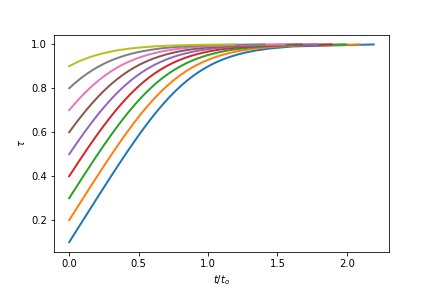
\includegraphics[width=0.45\textwidth, keepaspectratio]{figures/analyticUp.png}
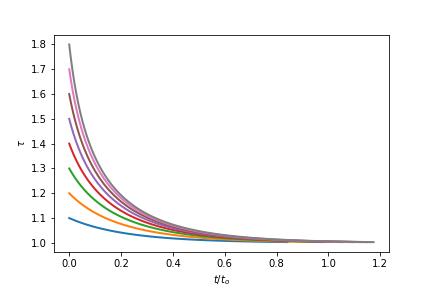
\includegraphics[width=0.45\textwidth, keepaspectratio]{figures/analyticDown.png}
\caption{The analytic solution for dimensionless temperature parameter $\tau(t) = T(t)/T_{eq}$
as a function of  dimensionless time parameter $t/t_o$ for initial conditions with $\tau_o<1$
(left) and $\tau_o>1$ (right). Note that in both cases $\tau(t)$ asymptotically approaches unity,
that is, $T(t)$ asymptotically approaches $T_{eq}$. 
\label{fig:analytic}}
\end{figure}



Equation~\ref{eq:dTdt} is typically solved using numerical integration. When the heat source is constant
in time, the solution can be obtained analytically. Equation~\ref{eq:dTdt} can be recast using 
eqs.~\ref{eq:Qout}  and \ref{eq:Teq} as 
\eq{
\label{eq:dtaudx}
               {d\tau \over dx }  = 1 - \tau^4, 
}
where $\tau=T/T_{eq}$, $x=t/t_o$ and the time scale $t_o$ is given by 
\eq{
\label{eq:t0}
     t_o =   { C m \over A_{tot} \, \epsilon_T \, \sigma \, T_{eq}^3}. 
}
The derivative $d\tau/ dx$ is positive when starting temperature $T_o=T(t=0)$ is
$T_o < T_{eq}$. Thus, when $Q_{in} = Q_{in}^{sun}$ and $T_{eq} = T_{eq}^{sun}$, the temperature
will be increasing with time, while for $Q_{in} = Q_{in}^{eclipse}$ and $T_{eq} = T_{eq}^{eclipse}$
the derivative is negative and the temperature decreases with time.

The simplified dimensionless differential equation \ref{eq:dtaudx} admits an implicit analytic 
solution:
\eq{
\label{eq:analytic}
{t \over t_o} = {1\over 2}\left[\arctan(\tau) - \arctan(\tau_o)\right] + {1\over 4}\left[\ln\left({\tau+1\over\tau_o+1}\right) - \ln\left({\tau-1\over\tau_o-1}\right) \right], 
}
where $\tau_o = T_o/T_{eq}$ is the initial condition. When $t \gg t_o$, $\tau$ asymptotically approaches unity. 
Figure~\ref{fig:analytic} illustrates solutions given by eq.~\ref{eq:analytic} for both $\tau_o<1$ and $\tau_o>1$. 



\subsection{Temperature variation for a bistable heat source} 


\begin{figure}[t]
\centering
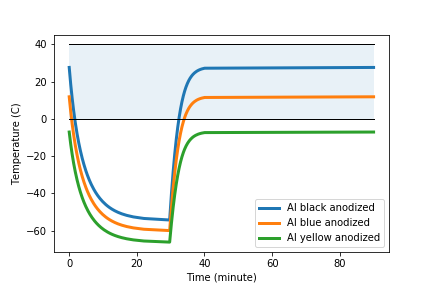
\includegraphics[width=0.31\textwidth, keepaspectratio]{figures/3tempsVStime_DefaultsMassVariationMsmall.png}
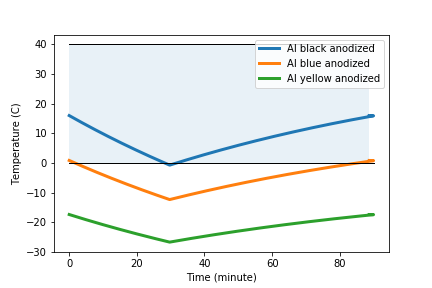
\includegraphics[width=0.31\textwidth, keepaspectratio]{figures/3tempsVStime_DefaultsMassVariationMdefault.png}
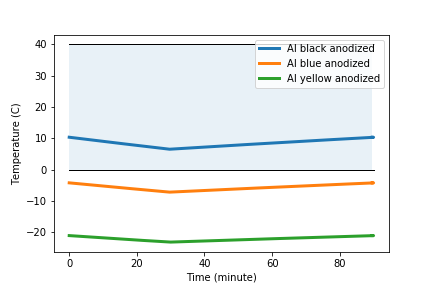
\includegraphics[width=0.31\textwidth, keepaspectratio]{figures/3tempsVStime_DefaultsMassVariationMlarge.png}
\caption{The satellite orbital temperature variation as a function of the surface emissivity properties 
and thermal inertia. The satellite total surface area is 0.1 m$^2$ (similar to 2U CubeSat), with 
effective absorptive surfaces corresponding to a spherical satellite. Three different types of anodized 
aluminum surfaces are modeled: black with $\alpha_S, \epsilon_T$  = (0.86, 0.86), blue: (0.67, 0.87)  
and yellow: (0.47, 0.87).  The thermal inertia is controlled by the satellite mass; left: low (0.05 kg), 
middle: medium (2.2 kg), right: high (10 kg). The temperature variation is compared to a typical battery operating 
temperature range (the blue horizontal band).  
\label{fig:Tt}}
\end{figure}


Now consider a bistable heat source, such as a satellite in an orbit and the heat source periodically
switching between $Q_{in}^{sun}$ and $Q_{in}^{eclipse}$. Because corresponding equilibrium temperatures 
$T_{eq}^{sun}$ and $T_{eq}^{eclipse}$ are different, the implied time scales for the temperature's return to its
equilibrium value, $t_o$ given by eq.~\ref{eq:t0}, will be different, too. Eq. ~\ref{eq:t0} implies that
the ratio of time scales in eclipse and when exposed to sunlight is 
\eq{
  { t_o^{eclipse} \over t_o^{sun} }= \left(Q_{in}^{sun} \over Q_{in}^{eclipse} \right)^{3/4} \approx 3. 
}

For a bistable heat source, the temperature at the end of the rising phase must be equal to the
temperature at the start of cooling phase and vice versa. As a result of this condition, the 
temperature will oscillate between two extremes, $T_{min}$ and $T_{max}$ with $T_{min} \ge T_{eq}^{eclipse}$ 
and $T_{max} \le T_{eq}^{sun}$.  Eq.~\ref{eq:analytic} appears too cumbersome to derive closed-form
analytic solutions for  $T_{min}$ and $T_{max}$; in practice,  $T_{min}$ and $T_{max}$ are easily determined
numerically (see Appendix B). 

When thermal inertia is vanishing, the temperature will return to its equilibrium values essentially
instantaneously and most of the time the satellite temperature will be either $T_{eq}^{eclipse}$ or $T_{eq}^{sun}$. 
On the other hand, for infinitely large thermal inertia the temperature will assume an equilibrium
value that corresponds to the heat source averaged over the satellite orbit. For example, if the satellite 
spends one third of the orbital period in eclipse, then
\eq{
\label{eq:TeqAve} 
      T_{eq}^{ave} = \left[ {1\over 3} \left(T_{eq}^{eclipse}\right)^4 +  {2\over 3} \left(T_{eq}^{sun}\right)^4 \right]^{1/4}. 
}
With $T_{eq}^{sun} = 301.1$ K and $T_{eq}^{eclipse} = 218.6$ K,  $T_{eq}^{ave}$ = 281.1 K  (7.9 $^\circ$C).  
With thermal inertia corresponding to heat capacity for aluminum ($C=921$ J\,kg$^{-1}$\,K$^{-1}$, see
Table~\ref{tab:inputsMatProp}), and satellite mass $m=2.0$ kg, the actual temperature extremes are $T_{min}$ = 272.4 K 
($-$0.8 $^\circ$C) and $T_{max}$ = 289.1 K  (16.0 $^\circ$C). Note that the $T_{max} - T_{min}$ difference  is about
five times smaller than the $T_{eq}^{sun}  - T_{eq}^{eclipse}$ difference. The variation of these extreme orbital 
temperatures on various input parameters is discussed next. 


\section{Numerical Examples} 

This section explores the impact of variations in input parameters on the mean satellite temperature and the 
amplitude of temperature variations.  The concept of hot and cold cases is also discussed. Note that numerical
values of various parameters were chosen to be similar to 2U CubeSat parameters; however, they do {\bf not}
correspond to any particular satellite. 

\begin{figure}[t]
\centering
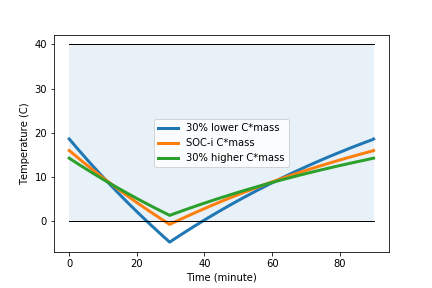
\includegraphics[width=0.45\textwidth, keepaspectratio]{figures/3tempsVStime_BlackAnodizedMassVariation.png}
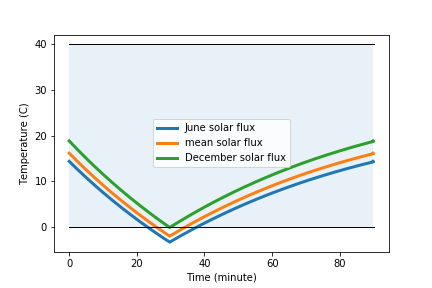
\includegraphics[width=0.45\textwidth, keepaspectratio]{figures/3tempsVStime_BlackAnodizedFsunVariation.png}
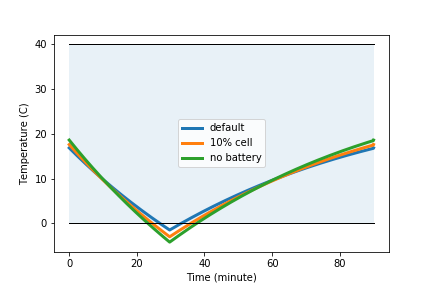
\includegraphics[width=0.45\textwidth, keepaspectratio]{figures/3tempsVStime_BlackAnodizedChargingVariation.png}
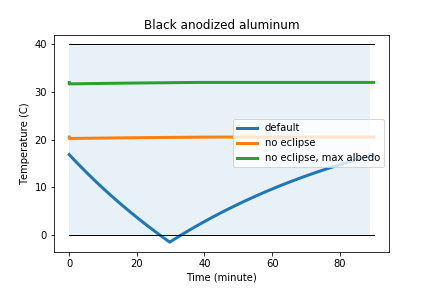
\includegraphics[width=0.45\textwidth, keepaspectratio]{figures/3tempsVStime_BlackAnodizedOrbitVariation.png}
\caption{The impact of thermal inertia (top left), solar flux variation (top right), solar cell efficiency (bottom left)
and the eclipse duration (bottom right) on satellite orbital temperature variation (all for black anodized aluminum 
surface with $\alpha_S, \epsilon_T$  = 0.86, 0.86). In the bottom left panel, it is assumed that a fraction of 
absorbed solar radiation is used to charge batteries, and it is then dissipated as heat at a constant rate
throughout the orbit. In the bottom right panel, the no eclipse case corresponds to a polar orbit whose normal
vector points to the Sun. The effective albedo is varied from 0.06 times its maximum value, as expected for such
an orbit, to 0.6 times its maximum value, as expected for an orbit that includes subsolar point. The temperature variation 
is compared to a typical battery operating temperature range (0--40 $^\circ$C, the blue horizontal band).  
\label{fig:Tt2}}
\end{figure}


\newpage
\subsection{The impact of thermal inertia on the amplitude of temperature variation} 

Figure~\ref{fig:Tt} shows the satellite orbital temperature variation as a function of the surface emissivity
properties and thermal inertia. The temperature variation is computed using analytic solution given by
eq.~\ref{eq:analytic} and emissivity properties corresponding to three different types of anodized aluminum 
surfaces (see figure caption). It is assumed that the orbital period is 90 min, with the eclipse portion lasting 
30 min. The aluminium heat capacity is assumed and the thermal inertia is controlled by the satellite mass. 

For low thermal inertia (left panel), the temperature displays large variation, drops quickly to the cold 
equilibrium temperature and rises back even faster to the hot equilibrium temperature. For very high
thermal inertia (right panel) the temperature varies by only a few degrees around the value given by 
eq.~\ref{eq:TeqAve} (7.9 $^\circ$C for black anodized Al surface). In the most realistic case shown in the 
middle panel, the temperature variation amplitude is 10--17 degrees, depending on the surface properties. 

This behavior is similar to potatoes taken from a hot oven: small satellites would cool faster 
than their scaled-up larger versions. However, here the difference in behavior is due to different 
thermal inertia for satellites that look identical from the outside (same size, shape and surface properties). 
Instead of small and large potatoes, a better analogy is solid and hollow potatoes of the same size.

It is important to recognize that some components within the satellite could achieve temperatures 
higher than $T_{max}$ (components close to the locations of internal power dissipation) but {\bf never
lower} than $T_{min}$  (assuming steady-state after many cycles). To obtain temperature variation for 
individual components, a professional tool (e.g., Thermal Desktop, Ansys) and detailed numerical 
computations need to be employed. Nevertheless, the essential impact of thermal inertia on the 
amplitude of temperature variation will remain. Perhaps the most important conclusion of this 
simplified analysis that pertains to detailed numerical modeling is that {\bf a full transient model
must be employed to assess the temperature variation} between $T_{min}$ and $T_{max}$. The 
extreme equilibrium temperatures, $T_{eq}^{sun}$ and $T_{eq}^{eclipse}$ are {\bf not} representative of the
actual temperature variation experienced by the satellite. 

In practice, the uncertainty in thermal inertia is much smaller than discussed in figure~\ref{fig:Tt}.
The top left panel in figure~\ref{fig:Tt2} shows that varying thermal inertia by $\pm$30\% 
around its mean value changes temperature predictions by about  5 $^\circ$C. 


\begin{figure}[t]
\centering
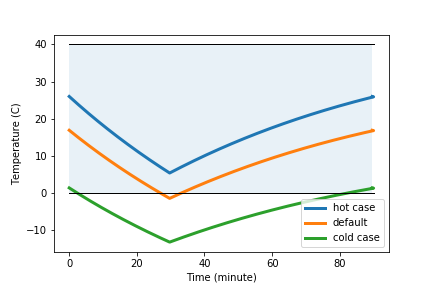
\includegraphics[width=0.45\textwidth, keepaspectratio]{figures/3tempsVStime_BlackAnodizedShotVScold.png}    
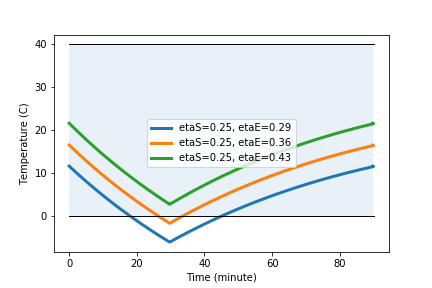
\includegraphics[width=0.45\textwidth, keepaspectratio]{figures/3tempsVStime_BlackAnodized2UareaVariation.png} 
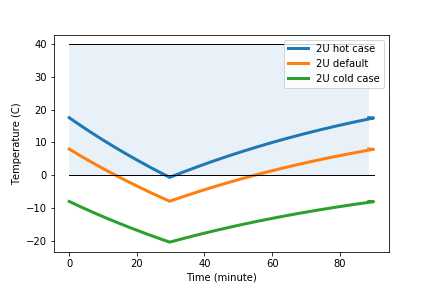
\includegraphics[width=0.45\textwidth, keepaspectratio]{figures/3tempsVStime_BlackAnodized2UhotVScold.png} 
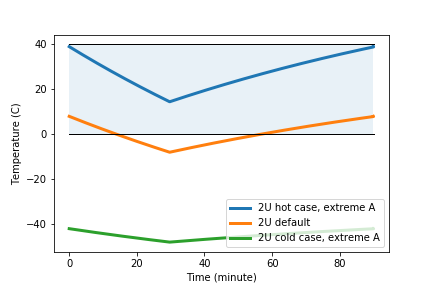
\includegraphics[width=0.45\textwidth, keepaspectratio]{figures/3tempsVStime_BlackAnodized2UhotVScoldExtreme.png} 

\caption{The impact of choosing extreme values of environmental conditions (top left), varying geometry expressed
through 20\% variation of the absorptive surface area (top right), extreme values of environmental conditions when 
assuming 2U CubeSat satellite geometry with randomized orientation (bottom left, $\eta_S=0.21$ and $\eta_E=0.36$), 
and with orientation that maximizes the temperature range between these so-called ``hot'' and ``cold'' cases (bottom
right, hot: $\eta_S=0.30$ and $\eta_E=0.38$; cold:  $\eta_S=0.10$ and $\eta_E=0.34$).  The temperature variation is 
compared to a typical battery operating temperature range (the blue horizontal band).  
\label{fig:Tt3}}
\end{figure}



\subsection{The impact of  variable solar flux on predicted satellite temperature} 

Due to Earth's elliptical orbit around the Sun, the solar flux at Earth's location varies by about 3.6\%
around its mean value, between its maximum at winter solstice and its minimum at summer solstice
(see Table~\ref{tab:inputsEnvParam}). The top right panel in figure~\ref{fig:Tt2} shows that this 
variation changes the minimum and maximum temperatures by about 3-4 degrees. 

 
\subsection{The impact of  battery charging on the amplitude of temperature variation} 

The energy spent to charge on-board batteries is converted to chemical energy and subtracted
from heat balance (see eq.~\ref{eq:dTdt}). It is returned to heat balance in the form of resistive
heat dissipation, at a constant rate as assumed here. Because the charging does not happen 
during the eclipsed portion of the orbit, this dissipation effectively ``flattens'' the heat source 
variation and decreases the amplitude of temperature variation. The bottom left panel in 
figure~\ref{fig:Tt2} shows that the conversion of 20\% of incoming solar flux to battery charge
and release as heat can decrease the amplitude of temperature variation by about 5 degrees
compared to no-battery case. 
 

\subsection{The impact of  eclipse duration on the amplitude of temperature variation} 

Given a fixed orbital period, the shorter is the eclipse the higher is the total accumulated
energy. The bottom right panel in figure~\ref{fig:Tt2} compares two polar orbits, one whose 
normal vector points to the Sun, with no eclipse, and another one that includes subsolar point
and has one third of orbital period spent in eclipse. The impact on mean temperature is about 
10-15 degrees. Uncertainties in effective albedo contribute to the uncertainty in predicted
temperatures; when
albedo is varied from 0.06 times its maximum value, as expected for the first orbit with
no eclipse, to 0.6 times its maximum value, the temperature is raised by another 10 degrees.


\subsection{The concept of hot and cold cases} 

Due to uncertainties in input parameters, including environmental, orbital and satellite parameters,
engineering pre-launch analysis often focuses on the most extreme scenarios that predict the coldest 
and the hottest satellite temperatures. 
 
The top left panel in figure~\ref{fig:Tt3} compares the cold and hot cases for a spherical satellite, 
with the extreme values of environmental parameters taken from Table~\ref{tab:inputsEnvParam}. 
The predicted temperature extremes differ by about 25 degrees.
 
The top right panel in figure~\ref{fig:Tt3} explores the impact of uncertainties in orbital parameters 
and satellite orientation by varying $\eta_E$ by 20\% around its mean value (about twice as much 
as typical uncertainties for a 2U CubeSat). The predicted temperature extremes differ by about 
10 degrees.

The bottom left panel is analogous to the top left panel, except that typical values of $\eta_S$
and $\eta_E$ for 2U CubeSat are used instead of values for a spherical satellite. 
Note that these parameters do {\bf not} correspond to any particular satellite.  
As expected, the predicted temperatures are about 8 $^\circ$C higher for the spherical satellite 
because of higher absorbed direct solar radiation. 

The bottom right panel in figure~\ref{fig:Tt3} pushes the comparison of hot and cold cases for 
2U CubeSat to its extreme. It is assumed that for hot case the satellite orientation is actively 
controlled so that during non-eclipsed portion its maximum possible projected area is always 
pointing towards the Sun, while during the eclipse it's pointed towards Earth (see figure caption). 
For cold case, the projected areas towards the Sun and Earth are minimized. The resulting
temperature extremes differ by as much as 80 degrees. It is noteworthy that it is possible
to reverse this scenario. If the satellite orientation is such that  the projected areas are
minimized for hot case, and maximized for cold case, the impact of environmental parameters 
can be reversed and hot case can be made colder than cold case. In other words, {\bf the satellite 
orientation can be more important than the variation of environmental parameters.} 



\section{Active temperature control \label{sec:active}} 

Given the allowed operating temperature ranges for satellite components (the most stringent requirement
comes from batteries, chosen here as 0--40 $^\circ$C for illustration), these results imply that 
low temperatures will be more worrisome than high temperatures. Motivated by this finding, we 
explored a model for active temperature control.

As a concrete satellite example, we used SOC-i CubeSat developed at the University of Washington. 
Adopted parameter values are discussed and listed in Appendix D. 


\subsection{A toy model for active temperature control } 

We developed a toy model for active temperature control that assumes an additional internal power 
dissipation whenever the satellite temperature drops below a pre-defined threshold. Analytic solution
given by eq.~\ref{eq:analytic} is not applicable any more because the time dependence of heat source
is now an unspecified function and numerical integration is used to obtain the solution\footnote{Python
code and Jupyter notebooks are publicly available at https://github.com/ivezic/CubeSats}. Analytic 
solution given by eq.~\ref{eq:analytic} was used to validate the numerical solution code in case of bistable 
heat source. 

We investigated cold case and three levels of power (2 W, 5, W, 10 W) that is applied whenever the temperature 
drops below 273 K (0 $^\circ$C). Results are shown in figure~\ref{fig:SOCi2}. 
Additional power can raise the satellite temperature by 5 to 11 degrees. The consumed power ranges
from 1.9 Wh to 4.3 Wh, and it is under the total available battery power (5.6 Wh for cold case and
$\eta_{cell}=0.2$; for hot, extreme case, it could be boosted to 18 Wh with $\eta_{cell}=0.3$). 
These results show that such an approach is a viable method for mitigating low temperatures.

\begin{figure}[t!]
\centering
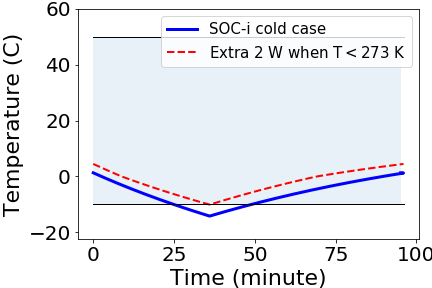
\includegraphics[width=0.3\textwidth, keepaspectratio]{figures/TempsPlotCompare_SOCi-cold-heated2.png} 
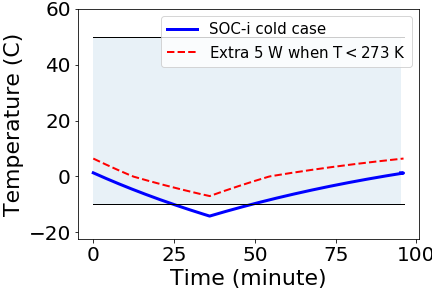
\includegraphics[width=0.3\textwidth, keepaspectratio]{figures/TempsPlotCompare_SOCi-cold-heated5.png} 
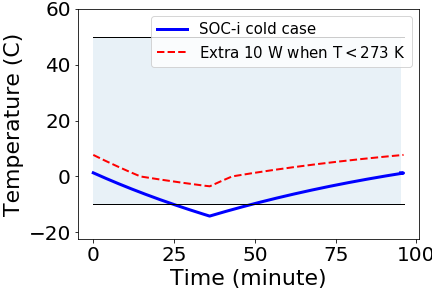
\includegraphics[width=0.3\textwidth, keepaspectratio]{figures/TempsPlotCompare_SOCi-cold-heated10.png} 
\caption{Illustration of the impact of active thermal control. A toy model assumes that whenever the satellite temperature
drops below zero $^\circ$C (273 K), an additional heating source with power of 2 W (left),  5 W (middle), or 10 W (right) contributes
to the heat balance. The blue lines correspond to the blue line in the left panel in figure~\ref{fig:SOCi1} (cold case) and the 
red dashed line is the corresponding temperature prediction with this additional heating power. The consumed power is about 
1.9 Wh, 3.4 Wh and 4.3 Wh, respectively (the total available battery power is 5.6 Wh). 
\label{fig:SOCi2}}
\end{figure}





\newpage
\section{Conclusions} 

When a body assumed to have a uniform temperature field is subjected to a bistable heat source,
there exists an analytic solution for the temperature variation with time. This simplified model is 
suitable for addressing a variety of satellite thermal analysis problems: studying the relative effects 
of surfaces with different emissivities, the effects of small changes in the solar flux between June 
and December, the impact of thermal inertia on predicted amplitude of temperature variation, and 
as a ``sanity check'' for the results obtained with numerical thermal models that utilize detailed 
geometrical and thermal descriptions of all satellite components. 

Brief examples of such studies are presented here. The most notable conclusions for further,
more detailed studies with numerical tools, include:
\begin{itemize}
\item The mean satellite temperature depends on the extreme values of steady-state equilibrium 
    temperatures for eclipsed and non-eclipsed parts of the orbit, and the duration of the eclipse
    relative to the orbital period (see eq.~\ref{eq:TeqAve}). 
\item The amplitude of temperature variation around the mean temperature is by and large 
     controlled by the satellite thermal inertia (see figure~\ref{fig:Tt}).
\item Although one might naively think that the satellite temperature is lower during the eclipse
    than when the satellite is exposed to direct sunlight, the satellite temperature range is {\bf identical} 
    for these two orbital phases because of cyclic boundary condition (unless the thermal inertia 
    is unrealistically low). 
\item Satellites with non-spherical geometry can be modeled within the same framework with 
    judiciously chosen effective surface areas, parametrized with $\eta_S$ and $\eta_E$
    (see eq.~\ref{eq:Qsun} and Appendix A). 
\item For non-spherical satellites, such as 2U CubeSat, the satellite orientation can have a
    significant impact on the predicted temperatures; indeed, with active 2U CubeSat orientation 
    control, the impact of environmental variations could be mitigated entirely (i.e., ``hot case'' 
    achieving lower temperatures than ``cold case''). 
\item {\bf Model uncertainties, including uncertainties in input parameters, result in uncertainties
   of predicted temperatures of at least 10 $^\circ$C!} 
\end{itemize} 

Since it appeared that low temperatures will be more concerning than high temperatures,
we also explored a toy model for active temperature control that assumes an additional internal 
power dissipation whenever the satellite temperature drops below a pre-defined threshold. 
We found out that such an approach is a viable method for mitigating low temperatures.

The latex source for this document, and the supporting python code for evaluating analytic and
numerical models and producing all the plots presented here, are publicly available\footnote{https://github.com/ivezic/CubeSats}. 


\vskip 0.2in 
%\newpage 
\leftline{\bf Acknowledgments} 
An initial version of the code for obtaining a numerical solution of the differential equation \ref{eq:dTdt} was 
contributed by Haley Stewart (University of Washington). I thank the University of Washington SOC-i team, in 
particular Boone Tate, Henry Brown and Charlie Kelly, for access to technical parameters describing their 
2U CubeSat named SOC-i. Without seeing their enthusiasm, I would have never written this paper. 
 

%\bibliographystyle{aasjournal}
%\bibliography{ref}{}
%\input{appendix}

\vskip 0.2in 
\leftline{\bf References}
Gilmore, D. 2002, ``Spacecraft Thermal Control Handbook: Fundamental Technologies'', 2nd ed. Aerospace Press 

Jacques, L. 2009, ``Thermal Design of the Oufti-1 Nanosatellite'', Master Thesis, University of Liege


%\newpage
\appendix{}

\vskip 0.2in
\leftline{\bf A. Effective area for the absorption of radiation from Earth}

\vskip 0.1in
 Effective area for the absorption of radiation from Earth can be computed using geometric radiative viewing factors
(and remembering that the factor $f_E$ is explicitly included in eq.~\ref{eq:Qref}). 

For a spherical satellite, 
\eq{
                  \eta_E  =  {1\over 2}  \left(1 - \sqrt{1- f_E} \right) \, f_E^{-1},
} 
where $f_E=[R_E/(R_E+h)]^2$, with Earth's radius $R_E=6,378$ km and $h$ is the satellite's altitude. As $h$
increases, $\eta_E$ for sphere varies from 1/2 to 1/4; for $h=550$ km, $\eta_E=0.36$.

For CubeSat satellites, $\eta_E$ can be obtained as the sum of values for all 6 sides because the viewing
factors are additive. For a flat surface whose normal is at angle $\beta$ relative to Earth's surface, 
\eq{
            \eta_E  = \cos(\beta), 
} 
for $|\beta|\le\arccos(\sqrt{f_E})$, and otherwise
\eq{
            \eta_E  = \pi^{-1} \left[ \left( \cos(\beta)\arccos(y) - x \,z \, \sin(\beta) \right) + f_E^{-1} \, \arctan(x^{-1} \, y \, \sin(\beta)) \right] 
} 
where $x=\sqrt{f_E^{-1}-1}$, $y=-x\tan(\beta)^{-1}$ and $z=\sqrt{1-y^2}$. The same expressions can
be used to compute $\eta_S$ for CubeSat satellites by setting $h$ to a very large value. 

For randomly oriented CubeSat satellites, $\eta_S \approx 0.21$ and $\eta_E \approx 0.36$ for both 1U and 2U versions,
with a scatter of about 10\% around these mean values for realistic orientations. For 2U CubeSat
with $h=550$ km, the possible ranges are  $\eta_S = 0.10 - 0.30$ and $\eta_E = 0.34 - 0.38$. 

\vskip 0.2in
\leftline{\bf B. A method for enforcing cyclic boundary condition for equation~\ref{eq:dTdt}}

\vskip 0.1in
Given the orbital period and eclipse duration, two cooling time scales $t_o$ (see eq.~\ref{eq:t0}) and two 
steady-state equilibrium temperatures $T_{eq}^{sun}$ and $T_{eq}^{eclipse}$, there are four unknowns to 
be solved for: $\tau_o^C$, $\tau_f^C$, $\tau_o^H$, and $\tau_f^H$, where $\tau=T/T_{eq}$, subscripts 
$o$ and $f$ correspond to the initial and final values, and superscripts $C$ and $H$ correspond to 
eclipsed and non-eclipsed parts of the orbit. 
 
Two equations come from the cyclic boundary condition that the final temperature for the $C$ phase
must be equal to the initial temperature for the $H$ phase, and vice versa
\eq{
\label{eq:taueqs}
     \tau_o^H = C_1 \,\tau_f^C \,\,  \,\,   {\rm and} \,\, \,\,   \tau_f^H = C_1 \, \tau_o^C,
} 
where $C_1 =  T_{eq}^{eclipse}/T_{eq}^{sun} \le 1$. The remaining two equations come
from applying eq.~\ref{eq:analytic} to $C$ and $H$ phases, where the left side is known and the right
hand side involves $\tau_o^C$ and $\tau_f^C$, and $\tau_o^H$ and $\tau_f^H$, respectively. 

After substituting eqs.~\ref{eq:taueqs} into two eqs.~\ref{eq:analytic}, the resulting system of 
two equations with two unknowns is easily solved numerically.  In case of numerical solution
for an arbitrary time dependence of the heating source, the cyclic boundary condition is satisfied
using iterations (usually only a few iterations are sufficient). 

%\vskip 0.2in
\newpage
\leftline{\bf C. Model parameters for the University of Washington SOC-i CubeSat}

The University of Washington SOC-i\footnote{A nod toward the Pacific Northwest salmon.}  
(the Satellite for Optimal Control and Imaging)  project\footnote{https://www.aa.washington.edu/news/article/2019-02-11/cubesat-team}
has a specific mission to demonstrate the ability to satisfy two constraints with its orientation
control and imaging systems. It was selected by NASA CubeSat Launch Initiative for launch in
2022 or 2023. We use it here as a specific example to quantitatively demonstrate the impact
of active temperature control on the satellite's minimum temperature. 

\vskip 0.1in 
\leftline{\bf Input satellite parameters}

We used the SOC-i CAD model\footnote{I am grateful to Boone Tate for extracting the model parameters.} 
developed for structural analysis to extract information about
external satellite surfaces and their material properties. We adopted the following description 
of external SOC-i surfaces: 
\begin{itemize}
\item  Top: 60\% solar panel, 40\% aluminum frame
\item  Bottom: 38\% aluminum frame, 62\% PCB (printed circuit board). 
\item  Sides (2): 64\% solar panels, 19\% aluminum panels (outside), 17\% aluminum frame rails
\item  Sides (2): 57\% solar panels, 26\% aluminum panels (outside), 17\% aluminum frame rails
\end{itemize}

With the values of absorptivity and emissivity listed in Table~\ref{tab:inputsAbsEmiss}, we obtained
their surface-weighted values $\alpha=0.83$ and $\epsilon=0.79$ (54\% of external surface area
is covered by solar panels). In addition, we assumed that the satellite mass is $m=2.6$ kg and 
adopted specific heat corresponding to aluminum ($C=768$  J\,kg$^{-1}$\,K$^{-1}$), yielding a
thermal intertia of $mC = 2.00$ kJ\,K$^{-1}$ (we note that a more accurate value of thermal inertia 
can be obtained by summing the $mC$ product for all individual structural components
in the SOC-i CAD model). 

\begin{table}[t]
	\centering
	\caption{Surface optical absorptivity and infrared emissivity for SOC-i surface materials. }
	\label{tab:inputsAbsEmiss}
	\begin{tabular}{r|r|r|r|r|r} % 
		\hline
  	              Part        &                Surface          &    $\alpha$  &   $\epsilon$    &   $k$ (W\,m$^{-1}$\,K$^{-1}$)   &  $C$ (J\,kg$^{-1}$\,K$^{-1}$)  \\
	  	\hline
         Solar panels        &       GaAs, with AR coating  &           0.92      &          0.85      &   60.6    &      324   \\  
     Al panels, outside   &     7075 Al, Kapton             &           0.87       &         0.81       &  121.2   &    801   \\ 
          Al frame rails    &       5052 Al, hard anodized &          0.86        &        0.86      &    138.5   &    768    \\  
                Al frame      &       5052 Al, alodine            &          0.08        &        0.15       &   138.5   &    768    \\
                PCBs            &               FR4                        &           0.81       &         0.90        &   18.0  &    1544  \\ 
 		\hline     
	\end{tabular} 
\end{table}
 

\vskip 0.1in 
\leftline{\bf Assumptions for orbital parameters}

It is already known that SOC-i will have a nearly-polar sun-synchronous 
orbit\footnote{See https://en.wikipedia.org/wiki/Sun-synchronous\_orbit} 
with an altitude of $h=550$ km and orbital inclination of 97.7 degrees. A satellite in sun-synchronous 
orbit passes over any given point of the planet's surface at the same local mean solar time because the 
orbit precesses through one complete revolution each year (that is, the orbit always maintains the same 
relationship with the Sun). 

The eclipse duration for sun-synchronous orbits depends on their right ascension of the 
ascending node (RAAN), which will not be known until the launch date (RAAN is determined
by the exact launch time). The orbital period for sun-synchronous orbit with an altitude of 
$h=550$ km is 96 mins, and the maximum eclipse duration is 36 mins.  When the orbital 
plane is perpendicular to incoming solar radiation, there is no eclipse (the satellite is following 
the terminator line at all times). 



\vskip 0.1in 
\leftline{\bf Hot and cold cases} 

We define ``hot'' and ``cold'' cases by first adopting 
the extreme values of environmental parameters from Table~\ref{tab:inputsEnvParam}. 
In addition, we make an assumption that the orientation of SOC-i's sun-synchronous orbit
results in an eclipse with maximum duration (36 min) for cold case, and no eclipse at all for 
hot case. 

The intensity of solar radiation reflected from Earth varies along the orbit. For a polar 
orbit passing through subsolar point, $f_{alb}=0.62$ for the non-eclipsed part of the orbit, while 
for a polar orbit aligned with the terminator (with no eclipse), $f_{alb}=0.06$. Therefore, 
we adopt $f_{alb}=0.62$ for hot case and $f_{alb}=0.06$ for cold case (note that reflected solar 
radiation contributes more flux for cold case, when not in eclipse). 
 
With these assumptions, we compute incoming heating flux.
For cold case, the only heating flux during the eclipsed portion of the orbit is IR flux from Earth. 
The variation of flux between hot and cold cases for three main heat sources is summarized in 
Table~\ref{tab:inputflux}. Note that reflected solar flux is smaller for hot case but this difference
is compensated by the absence of eclipsed orbital portion in hot case. 

Table~\ref{tab:inputflux} lists absorbed flux per unit area, assuming SOC-i's effective 
absorption coefficient ($\alpha$). The listed value are also appropriate for detailed 
Ansys-based modeling, but need to be corrected for $\alpha$ of each surface material.
The actual absorbed power (absorbed energy per unit time) depends on 
the values of $\eta_S$ and $\eta_E$, which in turn depend on orientation. We make additional 
assumptions about satellite orientation, as discussed next. 

\begin{table}[t]
	\centering
	\caption{Absorbed flux ($\alpha=0.83$) for hot and cold cases (in  Wm$^{-2}$). }
	\label{tab:inputflux}
	\begin{tabular}{r|r|r|r} % 
		\hline
  	                    Quantity  & hot case   &   cold  case &   ratio hot/cold    \\
		\hline
              Direct solar flux    &    1181        &     1098         &     1.08       \\
           Reflected solar flux  &     21.0        &     144.2        &     0.15     \\    
                       Earth IR flux  &   174.6       &     147.8        &     1.18      \\
		\hline
	\end{tabular} 
\end{table}



\vskip 0.1in 
\leftline{\bf Assumptions for satellite orientation}

The satellite orientation determines effective surface areas for the absorption of radiation from 
the Sun and Earth. For convenience, these surface areas are expressed relative to the total surface area, $A_{tot}$
(=0.1 m$^2$ for SOC-i), using $\eta$ factors ($\eta_S$ and $\eta_E$, respectively).  
We used results discussed in Section 2.4 to adopt the following values for SOC-i.

When averaged over plausible orientations and orbits, $\eta_S = 0.21$ and $\eta_E = 0.36$, 
with an uncertainty due to actual orbit specifics of the order 10\%. The limits of 
possible ranges are  $\eta_S = 0.10 - 0.30$ and $\eta_E = 0.34 - 0.38$. The limits for 
$\eta_S$ reflect the range of projected area towards plane-parallel rays for 2U CubeSat geometry, 
with the minimum value corresponding to one small side oriented perpendicularly to the incoming 
solar radiation. For $\eta_E$, the variation is much smaller because typically all six sides can 
``see'' Earth's surface\footnote{We note that even for spherical geometry $\eta_S$ and $\eta_E$
are generally different:  $\eta_S=1/4$, while $\eta_E$ decreases from 1/2 to 1/4 as the orbit
altitude varies from zero to infinity.}. 
 
We do not adopt specific satellite orientation for hot and cold cases but instead explore two 
options in each case.  First, we adopt averaged orientations for both hot and cold cases,
with $\eta_S = 0.21$ and $\eta_E = 0.36$ corresponding to 2U CubeSat values. As the second 
assumption, we consider the following extreme cases: $\eta_S = 0.30$ and $\eta_E = 0.34$ for 
hot case, and $\eta_S = 0.10$ and $\eta_E = 0.38$ for cold case.  
 
The second set of values assumes that the satellite orientation is actively controlled.  For hot
case, the maximum possible projected satellite area for plane-parallel rays is always pointing 
towards the Sun ($\eta_S = 0.30$). For cold case and during non-eclipsed portion, the smallest 
satellite side is always pointing towards the Sun ($\eta_S = 0.10$).  The adopted values of 
$\eta_E$ are its extreme values. 

 
\vskip 0.1in 
\leftline{\bf Assumptions for internal power dissipation}


A fraction of absorbed optical flux (the sum of direct solar flux and reflected solar flux) is often 
used to charge on-board batteries. We assume that 20\% of absorbed flux\footnote{Here, $\eta_{cell}$ 
represents the fraction of all absorbed radiation that was converted to battery charge. For example, if 
the cells occupy 2/3 of all external surfaces, and the cell conversion efficiency is 30\%, then $\eta_{cell}$= 0.2. 
For randomized orientiations, it's only ``effective'' quantities that count in the model considered here; 
however, when a specific satellite orientation is known, one could incorporate information about where 
exactly the solar cell panels are positioned, too.} is converted into chemical
energy ($\eta_{cell}=0.2$). This energy is returned back at a constant rate as internal heat dissipation. 

In hot case, satellite is always exposed to the Sun and there is {\bf no net effect} within the context
of single-temperature model considered here. In reality, and in detailed Ansys models, this
internal heat dissipation can modify the temperature distribution within the satellite (areas closer
to the heater will have elevated temperature). In cold case, the effect of internal heat dissipation
is to {\bf minimize} the amplitude of temperature variation, or equivalently, to {\bf raise the minimum
temperature} (at the end of eclipsed portion). 
 
These assumptions complete the specification of SOC-i hot and cold thermal models.  

\begin{table}[t]
	\centering
	\caption{Absorbed power (in Watt) and equilibrium temperatures for hot and cold SOC-i cases. }
	\label{tab:powertemp}
	\begin{tabular}{r|r|r|r|r} % 
		\hline
  	                    Quantity          & hot, random   &  hot, extreme &   cold, random  & cold, extreme   \\
		\hline
           Absorbed direct solar         &  24.8        &  36.6     &  23.1         &  11.0      \\
           Absorbed Earth albedo       &    0.8        &    0.8   &     5.2           &  4.9      \\    
               Absorbed Earth IR           &    6.3        &    6.6     &     5.3        &  5.0     \\
             Internal dissipation           &    5.1        &   7.5     &     3.5         &  2.0     \\
		\hline 
             Total input in eclipse       &     ---      &   ---   &     8.9       &    7.0  \\
              Total input in sun            &    31.8      &   44.0  &   31.4        &  19.7  \\
		\hline
              Equilibrium T in eclipse  &     ---     &    ---   &    211       &   199 \\
              Equilibrium T in sun       &      290      &   315   &    289        &  257  \\
 		\hline
                    $T_{min}$  (K)               &      290      &   315   &   259       &  235  \\
                   $T_{max}$  (K)               &      290      &   315   &   274        &  244  \\
		\hline
                    $T_{min}$  ($^\circ$C)   &       16.7         &  41.5             &  {\bf   $-$14.2  }  &  {\bf  $-$37.6}  \\
                   $T_{max}$  ($^\circ$C)    &  {\bf  16.7  }  &    {\bf  41.5}  &        1.3      &  $-$28.9   \\
		\hline
	\end{tabular} 
\end{table}

 


\vskip 0.1in 
\leftline{\bf Predicted absorbed power and equilibrium temperatures for hot and cold cases} 


Given all the input assumptions described above, it is straightforward to solve the
governing equation with direct numerical integration. Table~\ref{tab:powertemp} lists predicted 
absorbed power for all four modeled cases.  We note that the total energy stored in batteries, and 
dissipated as heat at a constant rate, ranges from 3.2 Wh for cold, extreme case to 12 Wh for hot, 
extreme case. 

\end{document}
 